

\documentclass[a4paper,10pt]{article}
\usepackage{listings,color,epsfig,amsmath,url}
\definecolor{codecolor}{rgb}{0.99,0.97,0.94} % color values Red, Green, Blue
\definecolor{commentcolor}{rgb}{0.1,0.5,0.1} % color values Red, Green, Blue
\definecolor{stringcolor}{rgb}{0.3,0.1,0.1} % color values Red, Green, Blue
\newcommand{\Code}[1]{\texttt{#1} }
\newcommand{\code}[1]{\Code{#1} }
\newcommand{\DB}   {\code{{MOOSDB}}}
\newcommand{\MA}   {\code{{MOOSApp}}}
\newcommand{\Ignore}[1]   {}



% Title Page
\title{Bridging Communities with \code{pMOOSBridge}}
\author{Paul Newman}



\begin{document}
\maketitle

\begin{center}

\epsfig{file=images/moose6.eps,width = 0.2\linewidth}
\end{center}
\begin{abstract}
This document will give you a description of how to use \code{pMOOSBridge} to link multiple MOOS communities together.
\end{abstract}

\section{Introduction}

\code{pMOOSBridge} is a powerful tool in building MOOS-derived
systems. It allows messages to pass between communities and is
able to rename the messages as they are shuffled between
communities. Many of the sections in this document rely on
\code{pMOOSBridge} to set up different communications topologies. There is no correct topology --- choose one that
works for your own needs.
\begin{figure}[ht]
\centering 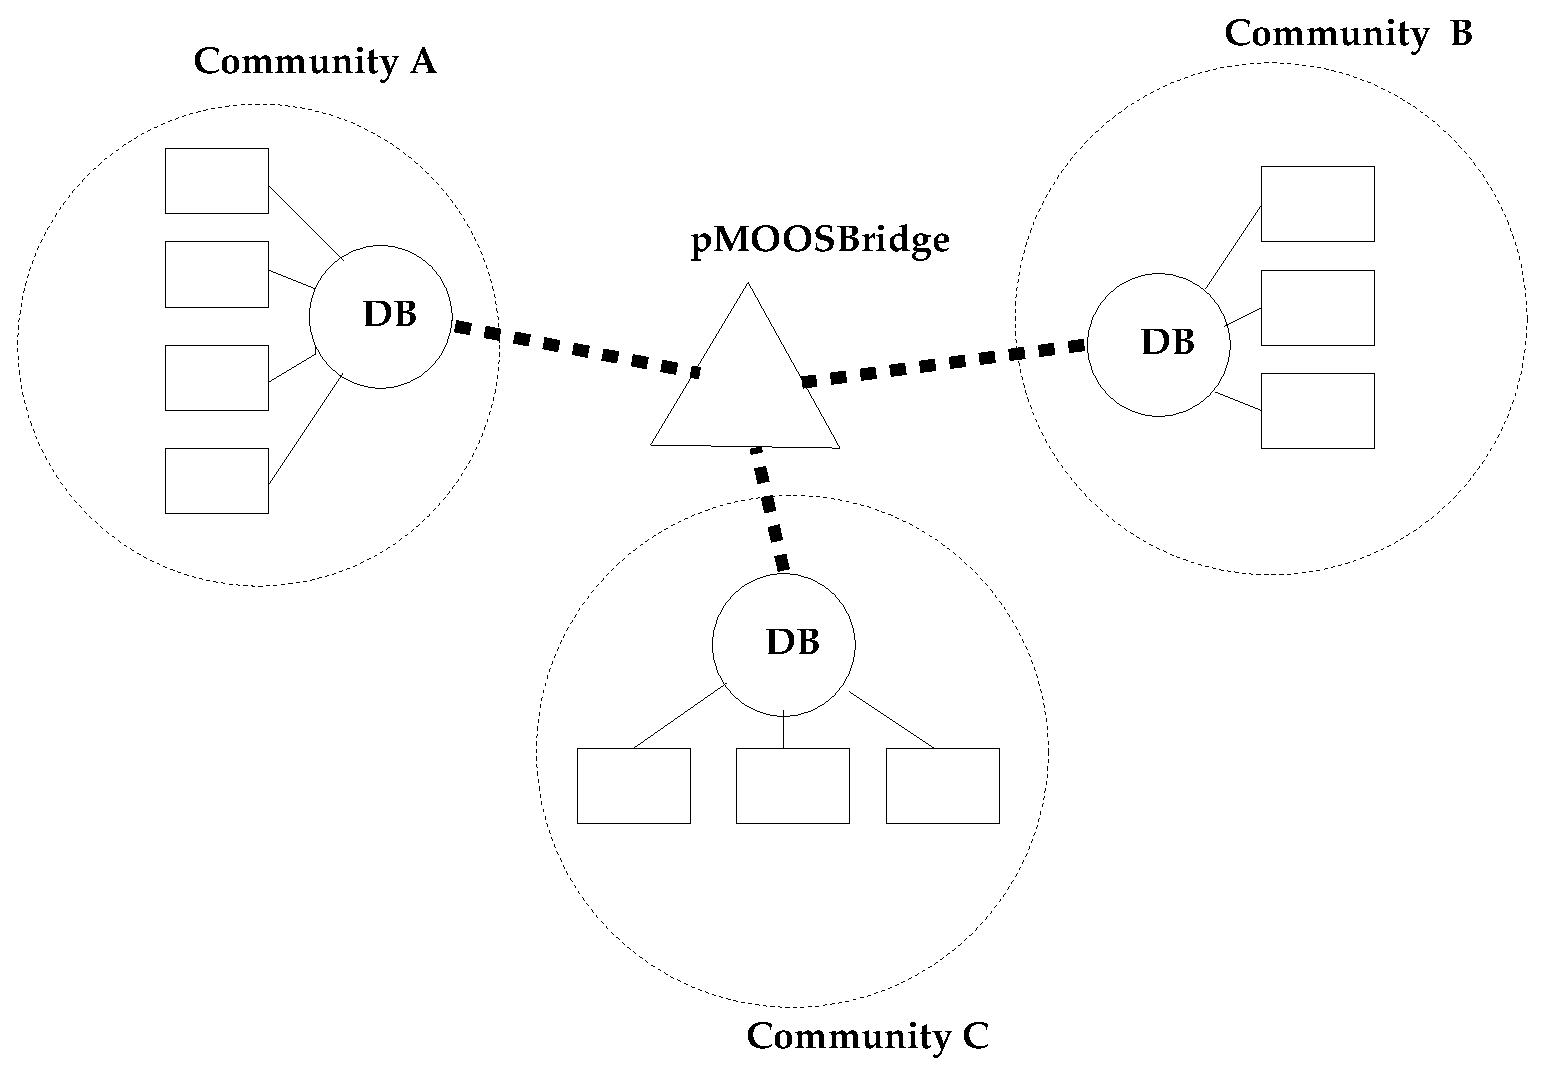
\epsfig{file = images/pMOOSBridge.eps , width = 0.6\linewidth}
\caption{A possible MOOSBridge
configuration. One instance of \code{pMOOSBridge} can ``talk'' to a limitless
number of communities. The configuration block specifies what
should be mapped or ``shared'' between communities and how it
should be done. The \code{SHARE} command specifies precisely what
variables should be shared between which communities.}\label{fig:MOOSBridge1}
\end{figure}
One instance of \code{pMOOSBridge} can ``talk'' to a limitless
number of communities. The configuration block specifies what
should be mapped or ``shared'' between communities and how it
should be done. The \code{SHARE} command specifies precisely what
variables should be shared between which communities and the
syntax is intuitive:\\

\code{SHARE= {\it{Comm@Host:Port[V1[,V2...]] $->$ Comm@Host:port
[V1,V2...]}}}\\

The triplet Comm@Host:Port is a description of a community ---  name and hostname/port pair. The community
description can be omitted on the LHS of the arrow, in which case the mission-file-scope defaults are assumed (see the example below).
Each variable (``V'') on the LHS (source) community will be inserted into the community on the RHS
If no variable names are specified on the RHS (destination) community the original names are used, otherwise
there is a one-to-one mapping between variable names on the LHS and new variable names (aliases) on the RHS. If however
there are more named shared variables than aliases, the variables for which an alias is not specified retain their original names.


For example\\
\begin{verbatim}
SHARE= VehA@nym.robots.ox.ac.uk:9000 [GPS_X]->VehB@kayak.mit.edu:9000 [GPS_X]
\end{verbatim}
Here the variable \code{GPS\_X} is shared between a community called ``VehA'', running from a \DB on the machine called
``nym.robots.ox.ac.uk'' listening on port 9000, is being inserted into a community called ``VehB'' using a \DB running on the machine called
``VehB@kayak.mit.edu'' also listening on port 9000. In both communities the variable is called ``GPS\_X''. However when viewed with
something like \code{uMS} (see the document on Graphical Tools) it can be seen that the \code{m\_sOrginatingCommunity} member of the \code{MOOSMsg}
carrying this data in the ``VehB'' commmunity will be ``VehA''.

\begin{verbatim}
SHARE= VehA@nym.robots.ox.ac.uk:9000 [GPS_X]->VehB@kayak.mit.edu:9000 [GPS_X_A]
\end{verbatim}
This is similar to the above example, only \code{pMOOSBridge} will rename ``GPS\_X'' to ``GPS\_X\_A'' in the
destination community. The next example shows how the source address need not be specified. When omitted the source community is
taken to be the community on which \code{pMOOSBridge} is running at the time. This example also shows how destination variable names may be omitted, in
which case the original (source community) variable name is preserved.
\begin{verbatim}
SHARE= [GPS_X]->VehB@kayak.mit.edu:9000
\end{verbatim}
Finally, more than one mapping can be specified in one line:
\begin{verbatim}
SHARE= [GPS_X,OVEN_TEMP]->VehB@kayak.mit.edu:9000 [GPS_X_A]
\end{verbatim}
Here GPS\_X is being mapped and renamed to \code{GPS\_X\_A} in community ``VehB'' but the variable \code{OVEN\_TEMP} is simply being shared without renaming.
It is important to realise that sharing is not bidirectional. In this case, a process notifying change in \code{GPS\_X\_A} in community ``VehB'' \emph{would not}
result in pMOOSBridge notifying the \DB in community ``VehA'' that ``GPS\_X'' has changed.


\begin{figure}[ht]
\centering 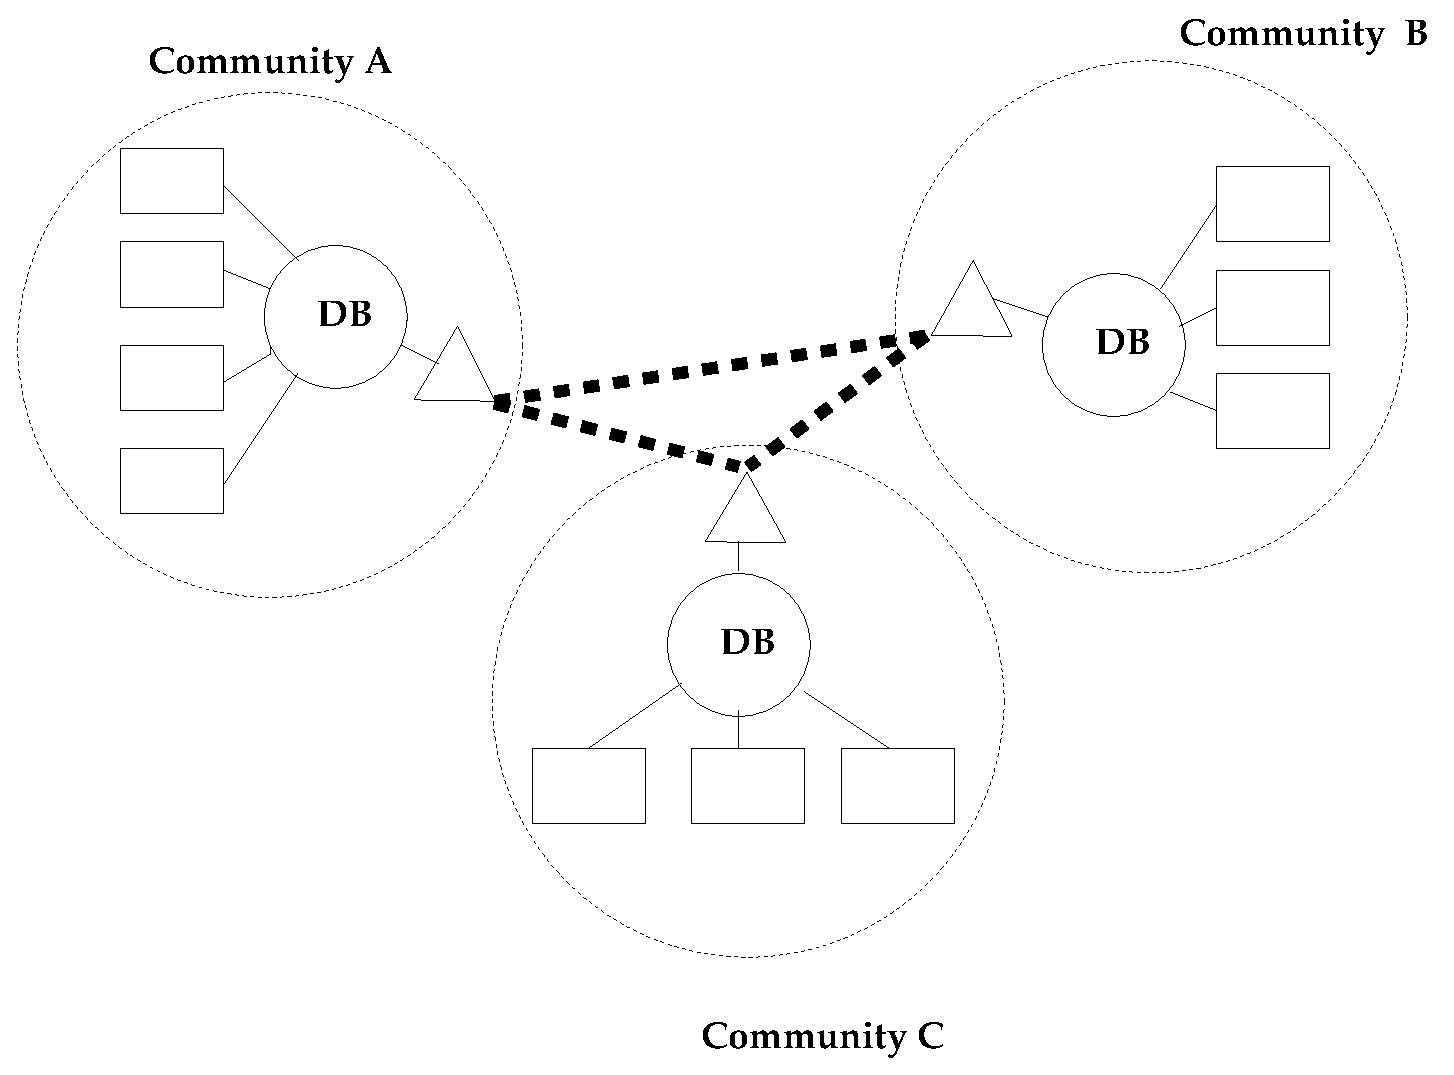
\epsfig{file = images/pMOOSBridge2.eps , width =
0.6\linewidth} \caption{An alternative MOOSBridge Configuration
--- one bridge per community. This may be preferable; it is undesirable to have one process manage all
the sharing of data. However it offers no \emph{functional} advantage over the topology shown in Figure
\ref{fig:MOOSBridge1}.}\label{fig:MOOSBridge2}
\end{figure}


\end{document} 